%% LICENCE: CC-BY-NC-SA
%% Copyright: Jesús Espino
%% Based on Git Internals chapter of ProGit book (http://git-scm.com/book)
\documentclass[10pt]{beamer}

\usepackage[utf8]{inputenc}
\usepackage[spanish]{babel}
\usepackage{graphicx}

\mode<presentation>
\usetheme{Madrid}
%\usecolortheme[RGB={111,73,135}]{structure}
\usecolortheme[RGB={128,0,0}]{structure}
%\usecolortheme[RGB={0,96,0}]{structure}
%\usecolortheme[RGB={200,0,200}]{structure}
%\usecolortheme[RGB={0,128,0}]{structure}
%\usecolortheme[RGB={0,0,128}]{structure}
\usefonttheme{serif}
\useinnertheme{rectangles}
\useoutertheme{split}

\setbeamercovered{transparent}

\title{Git Internals}
\author{Jesús Espino García}
\date{11 de Abril de 2013}
\subject{Git Internals}

\institute[Kaleidos]{
\includegraphics[height=1.5cm]{kaleidos.png}}

\setcounter{tocdepth}{2}

\AtBeginSubsection[]
{
  \begin{frame}<beamer>{Indice}
    \tableofcontents[sectionstyle=show/shaded,subsectionstyle=show/shaded/hide]
  \end{frame}
}

\begin{document}

  \frame{\maketitle}

  \section*{Introducción}

  \begin{frame}
    \frametitle{¿Por qué?}
    \begin{itemize}
      \item La interfaz de git es de bajo nivel.
      \item Conocer git bien da mucho poder.
      \item El poder está ahí aunque no lo conozcamos.
      \item Un gran poder conlleva una gran responsabilidad.
    \end{itemize}
  \end{frame}

  \begin{frame}
    \frametitle{Conceptos básicos}
    \begin{itemize}
        \item Procelain (Porcelana).
        \item Plumbing (Cañerias).
        \item Objetos
        \item Referencias
        \item Head
        \item Working copy
    \end{itemize}
  \end{frame}

  \begin{frame}
    \frametitle{Contenido de .git}
    \begin{itemize}
        \item Ficheros.
        \begin{itemize}
            \item HEAD
            \item index
            \item config
        \end{itemize}
        \item Directorios.
        \begin{itemize}
            \item objects
            \item refs
            \item hooks
            \item info
        \end{itemize}
    \end{itemize}
  \end{frame}

  \section*{Objetos}

  \begin{frame}
    \frametitle{Objetos}
    \begin{itemize}
        \item Bloque de datos almacenado en git
        \item Referenciado por el sha1 de su contenido
        \item Almacenados en el directorio .git/objects/ (o en packs).
        \item Hay 4 tipos de objetos en git (blob, tree, commit, tag).
    \end{itemize}
  \end{frame}

  \begin{frame}
    \frametitle{blobs}
    \begin{itemize}
        \item Será el nodo hoja de nuestros arboles.
        \item Será equivalente (normalmente) a nuestros ficheros.
    \end{itemize}
  \end{frame}

  \begin{frame}
    \frametitle{trees}
    \begin{itemize}
        \item Es un directorio de referencias a blob y otros trees.
        \item Almacena referencias (sha1 de objetos) y metadatos.
    \end{itemize}
  \end{frame}

  \begin{frame}
    \frametitle{diagrama de ejemplo de trees}
    \begin{center}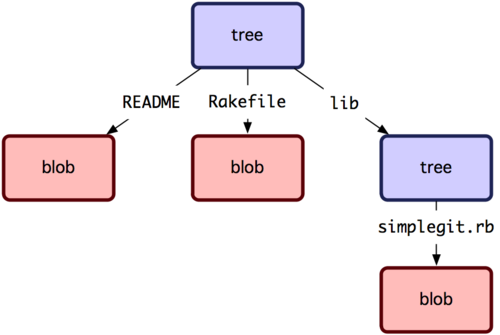
\includegraphics{trees.png}\end{center}
  \end{frame}

  \begin{frame}
    \frametitle{commits}
    \begin{itemize}
        \item Almacena una referencia a un tree.
        \item Almacena una referencia a su commit padre.
        \item Almacena metadatos del commit (autor, fecha, mensaje...)
    \end{itemize}
  \end{frame}

  \begin{frame}
    \frametitle{diagrama de ejemplo de commits}
    \begin{center}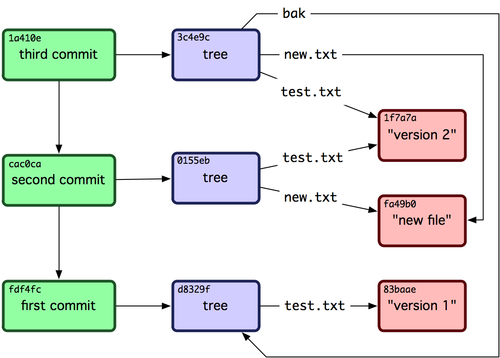
\includegraphics{commits.png}\end{center}
  \end{frame}

  \begin{frame}
    \frametitle{commits}
    \begin{itemize}
        \item Almacena una referencia a un commit.
        \item Almacena metadatos del commit (autor, fecha, nombre...)
    \end{itemize}
  \end{frame}


  \begin{frame}
    \frametitle{Objects storage}
    \begin{itemize}
        \item Se añade una cabecera con el tipo de objeto y la longitud del mismo.
        \item Se concatena con los datos que se van a almacenar
        \item Se calcula su sha1 que se utilizara como nombre del objeto.
        \item Se comprime con zlib.
        \item Se almacena en .git/objects/XX/XXXXXX\dots{}
    \end{itemize}
  \end{frame}


  \begin{frame}
    \frametitle{Ejemplos}
    \begin{itemize}
        \item git init repo; cd repo
        \item echo "Version 1" > fichero.txt; git add fichero.txt
        \item git commit -m "Version 1"
        \item ls .git/objects/*/*
        \item git cat-file -p HEAD
        \item git cat-file -p b7c0dba424af1e98a3570f8125476126129e5c32
        \item git cat-file -p fb8247c7b27ae4cad9e7e3e66ba95126658ea7c2
        \item cat .git/objects/fb/8247c7b27ae4cad9e7e3e66ba95126658ea7c2 | zlib-flate -uncompress
    \end{itemize}
  \end{frame}

  \section*{Packfiles}

  \begin{frame}
    \frametitle{Packfiles}
    \begin{itemize}
        \item Paquetes de objetos.
        \item Periodicamente git empaqueta los objetos en packs (gc).
        \item Se almacenan en .git/objects/pack/.
        \item Hay un listado de packs en .git/objects/info/packs.
        \item Cada pack tiene su indice en .git/objects/pack/.
    \end{itemize}
  \end{frame}

  \section*{Referencias}

  \begin{frame}
    \frametitle{Referencias}
    \begin{itemize}
        \item Están en .git/refs principalmente.
        \item Son punteros a objetos.
        \item Son ficheros contenidos en el directorio .git/refs
        \item Contienen el id del objeto al que apuntan.
    \end{itemize}
  \end{frame}

  \begin{frame}
    \frametitle{branchs}
    \begin{itemize}
        \item Están en .git/refs/heads
    \end{itemize}
  \end{frame}

  \begin{frame}
    \frametitle{HEAD}
    \begin{itemize}
        \item Esta en .git/HEAD
        \item Es una referencia simbolica que apunta a la referencia de la rama actual.
    \end{itemize}
  \end{frame}

  \begin{frame}
    \frametitle{tags}
    \begin{itemize}
        \item Están en .git/refs/tags
        \item Son referencias a commits o a objetos tag.
        \item Los tags simples son una referencia directa a un commit.
        \item Los tags con anotaciones son referencias a un objeto tag que apunta a un commit.
    \end{itemize}
  \end{frame}

  \begin{frame}
    \frametitle{remotes}
    \begin{itemize}
        \item Están en .git/refs/remotes
        \item Contiene las referencias de mis remotes.
        \item Se actualizan cuando hago push o fetch.
    \end{itemize}
  \end{frame}

  \begin{frame}
    \frametitle{Refspects}
    \begin{itemize}
        \item Forma de definir la relación entre las referencias de diferentes origines
        \item Tienen el formato [+]<src>:<dst>
        \item Opcionalmente se pone un + para actualizar la referencia cuando no hay fast-forward.
        \item Las referencias pueden tener * para definir "todo lo que haya en un directorio"
        \item No se permite el uso de * para selecciones parciales de referencias.
        \item Ejemplo: +refs/heads/*:refs/remotes/origin/*
    \end{itemize}
  \end{frame}

  \begin{frame}
    \frametitle{Pulling with refspects}
    \begin{itemize}
        \item Ejemplo: git fetch origin master:refs/remotes/origin/mymaster
        \item Descarga la referencia master del origin a refs/remotes/origin/mymaster en local
    \end{itemize}
  \end{frame}

  \begin{frame}
    \frametitle{Pushing with refspects}
    \begin{itemize}
        \item Ejemplo: git push origin master:refs/heads/qa/master
        \item Envia la referencia master local al refs/heads/qa/master en origin
    \end{itemize}
  \end{frame}

  \begin{frame}
    \frametitle{Borrando referencias}
    \begin{itemize}
        \item Ejemplo: git push origin :topic
        \item Borra la referencia topic en origin
    \end{itemize}
  \end{frame}

  \section*{Hablemos de algunos comandos}

  \begin{frame}
    \frametitle{init}
    Crea un .git con datos básicos.
    \begin{itemize}
      \item Un fichero config por defecto
      \item Los directorios refs, objects e info
      \item Un HEAD apuntando a la referencia master
      \item Y poco más
    \end{itemize}
  \end{frame}

  \begin{frame}
    \frametitle{add}
    \begin{itemize}
      \item añade el fichero a la base de datos de Objetos
      \item añade el fichero al index
    \end{itemize}
  \end{frame}

  \begin{frame}
    \frametitle{commit}
    \begin{itemize}
      \item Añade el tree apuntando al arbol de ficheros al que apunte el index a la base de datos de Objetos
      \item Añade el commit apunte al tree recien añadido a la base de datos de objetos
      \item modifica el HEAD
      \item modifica la referencia de la rama actual
    \end{itemize}
  \end{frame}

  \begin{frame}
    \frametitle{push}
  \end{frame}

  \begin{frame}
    \frametitle{fetch}
  \end{frame}

  \begin{frame}
    \frametitle{reset}
  \end{frame}

  \begin{frame}
    \frametitle{checkout}
  \end{frame}

  \section*{Para terminar}

  \begin{frame}
    \frametitle{¿De qué no hemos hablado?}
    \begin{itemize}
        \item Más comandos de porcelana.
        \item Comandos de plumbing.
        \item Protocolos de transferencia.
        \item Mantenimiento y recuperación de datos.
        \item Stash
    \end{itemize}
  \end{frame}

  \begin{frame}
    \frametitle{Referencias}
    \begin{itemize}
      \item \small{http://git-scm.com/ - Web oficial de git.}
      \item \small{http://git-scm.com/book - ProGit (El libro de Git).}
      \item \small{http://gitguys.com/ - Página sobre git.}
      \item \small{http://github.com/ - Servicio de git por excelencia.}
      \item \small{http://bitbucket.org/ - Servicio de git de repositorios privados gratis.}
    \end{itemize}
  \end{frame}

  \begin{frame}
    \frametitle{Dudas}
    \dots
  \end{frame}

\end{document}
